% ======================================================================================================
% NOTES, TODOS
% ======================================================================================================
\subsection{Search Result and Bibliometric Analysis}

After completion of the selection process, which involved applying inclusion and exclusion criteria and eliminating duplicate studies, a total of 69 research papers were considered eligible for further review and analysis. The accompanying pie chart (see Figure \ref{fig:archive-itemtype}) reveals that IEEE was the primary publisher of the selected papers, accounting for 44 of them. SpringerLink was the second largest contributor, with 13 publications, while Elsevier (5), ACM (4), MDPI (2), and IOS Press(1) each account for the lowest contribution of publications. The second right side of the pie chart \ref{fig:archive-itemtype} also demonstrates that the majority of the selected papers were sourced from Web of Science and Scopus, followed by IEEE and SpringerLink. The distribution of publication types among the 73 selected papers is worth nothing. Of these papers, 60\% (i.e., 44 papers) were published as conference papers, whereas the remaining 40\% (i.e., 29 papers) were in the form of journal articles.



% \begin{figure}
% \includesvg[width=0.5\textwidth]{images/svg/databases.svg}
% \includesvg[width=0.5\textwidth]{images/svg/itemtype.svg}
% \svgcaption{This is the label for the SVG image.}
% \label{fig:image}
% \end{figure}

\begin{figure}[H]    
    \caption{An Analysis of Paper Distribution Based on Source and Publisher.}
    % \centring
    \begin{subfigure}[b]{0.45\textwidth}
    \caption{Number of selected papers per publisher.}
        \includegraphics[width=\textwidth]{images/newimages/publisher-per-paper-screenshot.png}
        % \includesvg[width=\textwidth]{images/svg/databases.svg}
    \end{subfigure}
    \begin{subfigure}[b]{0.45\textwidth}
    \caption{Number of selected papers per source.}
        \includegraphics[width=\textwidth]{images/newimages/source-paper-screenshot.png}
        % \includesvg[width=\textwidth]{images/svg/itemtype.svg}
    \end{subfigure}
    \label{fig:archive-itemtype}
\end{figure}
 
Analysis of the distribution of selected papers based on publication year revealed that the majority of articles were published in 2022 and 2021 (see Figure \ref{fig:bar-chart-yaer}). Furthermore, the bar chart illustrates a general upward trend in the number of publications addressing security concerns for industries utilising Digital Twin and (I)IoT applications. This trend indicates that there is a growing interest and concern among researchers in the field of Digital Twin and (I)IoT security, and highlights the relevance of this systematic literature review.

\begin{figure}[H]    
    \caption{Yearly Publication Statistics: Investigating the Number of Papers Published}
    % \includesvg[width=0.9\textwidth]{images/svg/pub_year_white_bg.svg}
    \includegraphics[width=\textwidth]{images/newimages/paper-per-yerapublished-v2.png}
    \label{fig:bar-chart-yaer}
\end{figure}

To gain a deeper understanding of the trending topics within the 69 selected papers published between 2018 and 2023, a frequency analysis of keywords was conducted. This analysis was performed by extracting keywords that appeared more than three times in the abstracts and keyword sections of the articles using the VOSviewer tool. Further filtering and sensitization was applied to create a shortlist of keywords. Additionally, keywords which have similar meanings with different spellings and variations were merged. 

The resulting frequency analysis of keywords, illustrated in Figure \ref{fig:alluvial-key}, provides valuable insight into the key themes and concepts that are prevalent in current research on the topic of DT and IoT security. This analysis can help guide future research by identifying areas where there is a need for further investigation and providing a sense of the current state of the field.


\begin{figure}[H]
    % \includesvg[width=0.9\textwidth]{images/svg/key_buble.svg}
    % 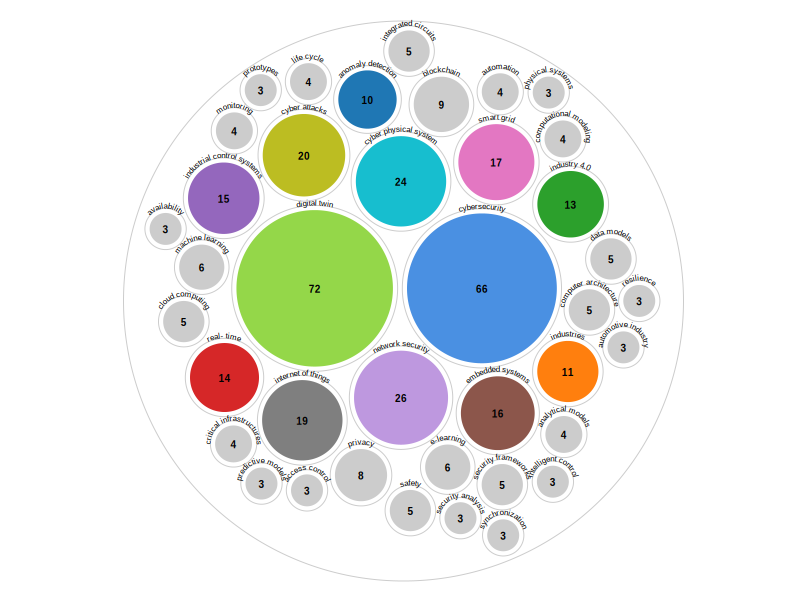
\includegraphics[width=\textwidth]{images/svg/key_buble.png}
    \caption{Frequency of keywords from keyword section of 69 papers}
    \includegraphics[width=0.8\textwidth]{images/newimages/vosviewer-keyword-occurance-vertical.png}
    \label{fig:alluvial-key}
\end{figure}
As was previously stated, in this study, 69 papers were analyzed to generate a list of 367 keywords using VOSViewer. During our analysis, we utilized a thesaurus text file to merge keywords with similar semantic meanings.

For instance, we replaced artificial intelligence with machine learning, and intrusion detection with anomaly detection. We also replace the occurrence of security by cybersecurity. Similarly, we combined control systems under the term industrial control system. We further streamlined our findings by using industry 4.0 as an umbrella term for smart manufacturing. Additionally, we have replaced the term "real-time" with "real-time system". 


The analysis of the selected papers using VOSviewer software revealed that which terms were frequently mentioned in the keyword section of the paper. The most frequently mentioned terms were "digital twin" with 72 occurrences, followed by "cybersecurity" with 66 occurrences, "cyberphysical system" with 24 occurrences, "cyber attacks" with 20 occurrences, "internet of things" with 19 occurrences, and "embedded systems" with 17 occurrences. This analysis highlights the key themes and concepts that are prevalent in current research on the topic of Digital Twin and IoT security. The high frequency of the term "digital twin" indicates the centrality of this concept in the field and the importance of understanding its role in ensuring the security of industries utilizing DT and IoT applications. The frequent mention of terms such as "cybersecurity" and "cyber attacks" further emphasizes the need for robust security measures to protect these systems from malicious actors. Additionally, the presence of terms such as "cyberphysical system" and "embedded systems" highlights the need for interdisciplinary research and collaboration between experts in fields such as computer science, engineering, and physics to effectively address the security challenges facing Digital Twin and IoT.

In order to gain further insights into the evolution of research in the field of Digital Twin and IoT security, a keyword co-relationship network analysis was extracted from the VOSviewer tool. This analysis aimed to identify clusters of related items and visualise the relationships between keywords over time. The results of this analysis revealed that in the early days of research on Digital Twin, keywords such as "computational modeling", "embedded system", "situational awareness", "safety", and "simulation"" were frequently mentioned, which suggests that the primary focus of research at that time was on utilising Digital Twin as a visual aiding tool. However, more recent research is characterized by the frequent mention of emerging technologies such as "blockchain," "machine learning," "e-learning" "5G," and "emulation" This indicates that the development of Digital Twin has shifted towards utilising these technologies and augment Digital Twin to provide more service other than used as a model.



\begin{figure}[H]
    % \centering    
    \caption{keyword co-relationship from VOSviewer}
    \includegraphics[width=\textwidth, center]{images/newimages/vosviewer-2oc.png}
    % \includesvg[width=\textwidth]{images/new}
    % \includesvg[inkscapelatex=false,width=0.95\columnwidth]{images/key_belt.svg}
    \label{fig:co-occurrence-vosv}
\end{figure}

The analysis of the co-occurrence of keywords in the selected articles, as represented in Figure \ref{fig:co-occurrence-vosv}, reveals the identification of eight clusters. These clusters, as defined by the VOSviewer documentation, are groups of terms that exhibit a high degree of relatedness. 

% Cluster one encompasses terms related to 5G technology, machine learning, real-time security analysis, security frameworks, access control, and automation, highlighting the importance of incorporating advanced technologies in the field of security and access control automation. This cluster also suggests a growing emphasis on real-time security analysis to ensure quick identification and response to potential threats.

% Cluster two comprises keywords such as cybersecurity, data models, digital twin, internet of things, privacy, prototypes, safety, and cloud computing. The inclusion of terms such as privacy, prototypes, and safety in this cluster indicates a growing concern for the protection of sensitive information and the security of digital representations of physical systems. 

% The third cluster encompasses terms such as those related to the automotive industry, availability, blockchain, industry 4.0, industrial control systems, system life cycles, intelligent control, software, and tools. This cluster suggests a growing emphasis on the use of blockchain technology for secure data management in the automotive industry for data sharing. 

% The fourth cluster is comprised of analytical models, anomaly detection, cyber-attacks, monitoring, resilience, critical infrastructure, integrated circuits, and physical systems. This cluster shows the association of identification and mitigation of potential security threats through the use of analytical models to detect anomalies to increase the resilience of critical infrastructure.

% The final cluster includes terms such as cyber-physical systems, e-learning, embedded systems, predictive models, and smart grids. This cluster highlight the importance of training and education to promote the secure use of cyber-physical system such as smart grids.

\textit{Cluster One:}
This cluster focuses on various aspects related to the industrial and digital domains. It includes topics such as authentication, autonomous vehicles, cloud computing, costs, digital twin, industrial internet of things (IIoT), microgrids, real-time systems resilience, and smart manufacturing. The common theme in this cluster appears to be the integration of digital technologies in industrial settings, emphasizing security, efficiency, and advanced manufacturing processes.

\textit{Cluster Two:}
This cluster revolves around computer-related topics, computational modelling, computer architecture, and embedded systems. It also includes subjects like cyber-physical systems, industry 4.0, network security, situational awareness, and smart grids. The primary focus here seems to be the intersection of computer science and engineering, with an emphasis on the integration of smart technologies into physical systems and networks.

\textit{Cluster Three:}
Cluster three is centered around security and privacy concerns in the digital landscape. It encompasses topics such as blockchain, cyber digital twin, cybersecurity, data privacy, safety, smart cities, smart contracts, soft sensors, and traffic control. The key theme here is the exploration of secure and privacy-preserving solutions in digital ecosystems, including blockchain technology and data protection measures.

\textit{Cluster Four:}
This cluster focuses on topics related to access control, automation, data security, and smart homes within the Internet of Things (IoT) context. The cluster includes items such as access control, automation, data security emulation, and IoT smart homes. The primary theme revolves around securing and managing access to IoT devices and systems, as well as exploring automation and smart home technologies.

\textit{Cluster Five:}
Cluster five centers on industrial control systems and security. It includes topics such as industrial control systems, integrated circuits, intelligent control, intrusion detection, machine learning, predictive models, and security-by-design. The focus here is on ensuring the security and reliability of industrial control systems, incorporating intelligent control algorithms, and leveraging machine learning for intrusion detection and predictive maintenance.

\textit{Cluster Six:}
This cluster encompasses topics related to communication networks and security frameworks. It includes items such as 5G, cyber range, industries, pipelines, security framework, security operation center, and wireless communication. The primary theme is the exploration of secure communication in various domains, including the development of security frameworks and the implementation of wireless communication technologies.

\textit{Cluster Seven:}
Cluster seven revolves around anomaly detection, cyber-physical systems, deep learning, monitoring, and SCADA systems. The focus here is on leveraging advanced techniques such as deep learning and anomaly detection for monitoring and securing cyber-physical systems, particularly in the context of SCADA systems.

\textit{Cluster Eight:}
Cluster eight is centered around analytical models, simulation, and testing. The focus is on the development and application of analytical models and simulation techniques for testing and evaluating various systems or scenarios.